\documentclass[12pt]{article}
\usepackage{graphicx}
\usepackage{amsmath,amssymb}
\usepackage{caption}
\usepackage{subcaption}
\usepackage{hyperref}
\usepackage{color}
\textheight 240mm
\textwidth  170mm
\oddsidemargin  0mm
\evensidemargin 0mm
\topmargin -20mm

\DeclareMathOperator*{\argmin}{argmin}
\DeclareMathOperator*{\argmax}{argmax}
\newcommand{\tss}[1]{\textsuperscript{#1}}

\hyphenpenalty = 9001 % Over 9000!!

\begin{document}
%_________________________________________________________________
\title{Automated Music Genre Classification}
\author{James Folberth, Dale Jennings, Alyson Fox}
\date{15 December, 2014}
\maketitle
%_________________________________________________________________
\section{Introduction}
%_________________________________________________________________
\indent Digital music has changed the face of music collection. Users can have a megabyte or a gigabyte worth of music on their personal laptops and can easily download music from the internet. This has lead to the need to invent and test new tools in musical information retrieval. There are many websites and apps, Pandora and iTunes are a few examples, that can create playlists based on similarity to a certain song or genre of music. These sites need to be able to classify certain features of a song and build the playlist from there.\\

The goal of this project is to classify the genre of a song. This may seem like a simple problem, since we can usually classify a song by ear, but that relies on the user having a vast knowledge of music. If we can automate the process using computers, we could find new and interesting insights that may not be obvious. However, this adds complexity that must be dealt with since we need techniques so that  the computer can ``listen'' to the song and extract features to be able to identify the genre. To do this we take  a song, which is a continuous signal and we sample at certain frequency to transform it into a discrete signal that is based on pitch which created by the sound pressures changes  and define it as a function of time. From the discrete signal we can define  ``features" for each song that may be able to be used to classify the genre.\\

 For our project we are only classifying within six different genres: classical, electronic, jazz/blues, metal/punk, rock/pop, and world. To compute similarities between each song it is imperative that we generate features. Given 729 training tracks, we will construct features for each song and the song that we would like to classify. We can use theses quantifiable features to develop a machine learning algorithm to classify the genre. Most features that we used were developed by or used in Elias Pampalk dissertation \cite{pampalk:dissertation} or in Tzanetakis and Cook \cite{tzanetakis:classification}.

%_________________________________________________________________
\section{Distance in song-space}
% TODO Dale's going to clean this up.

When trying to define a distance in song-space for genre classification, it is not very helpful to try to construct a distance based solely on the raw data.  Instead, feature extraction is applied to the songs in an attempt to represent each song in a manner that is more similar to how the human ear and brain perceives songs.  Having this quantification of musical features allows songs to be classified in a manner more similar to how a human might classify the songs.

\subsection{Preprocessing}

One step in feature extraction is in preprocessing the song, where the raw pulse code modulation form of the song is transformed into segments of spectral information.  The preprocessing improves the accessibility of the features and is also the first step in dimensionality reduction.

\subsubsection{Power Spectrum}
The power spectrum of an audio signal is a frequency-domain representation of the signal.  More specifically, we use a short-time Fourier transform to transform the signal to the frequency-domain, while maintaining some temporal locality.  The signal is broken up into many small, possibly overlapping segments, each of which then is windowed and passed through a Fourier transform.  Once in the frequency domain, the square magnitude is calculated, to get the power spectrum.

\subsubsection{Mel Frequency Cepstrum}
While the power spectrum of a signal presents some nice information of the signal, the human ear processes audio signals in a different manner.  The Mel Frequency Cepstrum is a way to transform the power spectrum into a scale that is more similar to how the human ear perceives the signal.  Specifically, the Mel-scale is defined to be
$$ m_{Mel} = 1127.01048 \ln(1 + f_{Hz}/700) $$
Instead of looking at a linear spread of frequencies, the Mel-scale frequencies are approximately linear for small (below 500Hz) frequencies and have a logarithmic spread for higher frequencies.  In order to transform the power spectrum into the Mel Frequency Cepstrum, triangular filters are applied to the power spectrum, binning the frequencies appropriately.\\

The frequency scales are not the only difference with how the ear perceives audio.  The loudness is also perceived in a non-linear way.  The perceived loudness of sounds approximately follows the Decibel (dB) logarithmic scale.  The logarithm of Mel power is calculated to convert to this dB representation.  Using the power spectrum in the Mel scale, we have various methods to compute a spectral similarity measure between songs.  There are also many other features that can be extracted from the Mel power spectrum.

\subsection{Temporal Features}
The first set of features that can extracted from a song are temporal features, that do not require any spectrum preprocessing.  These features are calculated over a moving window for the entire song.  In order to capture the distribution of each of these temporal features, the first four moments (mean, variance, skewness, and kurtosis) are calculated and stored.  For details on the calculations and meaning of each of these temporal features, refer to \cite{lerch:aca}.

\begin{itemize}
\item Autocorrelation Coefficients
\item Autocorrelation Maximum
\item Peak Envelope
\item Predictivity Ratio
\item Root Mean Square
\item Standard Deviation
\item Zero Crossing Rate
\end{itemize}

\subsection{Spectral Features}
The next set of features require the previously discussed preprocessing steps.  These features are considered spectral features, as they rely on the spectrum, or Mel cepstrum, of the song.  As with the temporal features, the spectral features are calculated over moving time windows, and in order to capture the distribution of these features, the first four moments are calculated and stored.  For details of the calculations and meaning, refer to \cite{lerch:aca} and \cite{pampalk:dissertation}.

\begin{itemize}
\item Spectral Centroid
\item Spectral Crest
\item Spectral Decrease
\item Spectral Flatness
\item Spectral Flux
\item Spectral Kurtosis
\item Spectral Rolloff
\item Spectral Skewness
\item Spectral Slope
\item Spectral Spread
\item Tonal Power Ratio
\item Mel Frequency Cepstrum Coefficients (1-13)
\item Pitch Chroma (12 notes)
\end{itemize}

%\subsection{Available Simple Features}
%
%After this preprocessing has been performed, many simpler features are easily extracted.  With these features, a distance can be constructed between songs, with the metric depending on which features are of interest.  Below, some of the possible features are described.  This list is in no way exhaustive, as many other features exist.
%
%\subsubsection{Zero Crossing Rate}
%
%The zero crossing rate (ZCR) is one of the easiest features to extract, as it does not require any preprocessing.  The ZCR measures the average number of times a signal crosses zero, normalized to some unit time.  Generally speaking the ZCR can be used to help classify the noisiness of a signal, although perceived noisiness and perceived ZCR may differ for certain signals (as noted in Pampalk's thesis).  Mathematically, the ZCR is given by
%$$ \text{zcr} = \frac{\sum_{i=1}^{N-1} \vert w_{i+1} - w_{i} \vert}{2 N f_s} $$
%where $\mathbf{w}$ is the raw data, $N$ is the length of the data, and $f_s$ is the sampling frequency.
%
%\subsubsection{Root Mean Square Energy}
%
%The Root Mean Square (RMS) energy is another feature that comes directly from the audio signal.  The RMS energy gives a measure of overall loudness of an audio signal, and is given by
%$$ \text{rms} = \sqrt{\frac{1}{N}\sum_{i=1}^N w_i^2} $$
%
%
%\subsubsection{Noisiness}
%
%As mentioned earlier, the ZCR gives one attempt at classifying noisiness, although it can differ from perceived noisiness.  To improve the measure of noisiness, the dB scale power spectrum of the audio signal can be used.  One measure of this spectrum based noisiness is based off of differences between frequency bins for a given time segment.  Let $\mathbf{P}$ represent the power spectrum of a signal, with rows corresponding to frequency bins, and columns corresponding to time segments.  Then,
%$$ \text{noisiness}  = \sum_{t} \sum_{f} \vert P_{f+1,t} - P_{f,t} \vert $$
%In practice, frequencies below 800Hz are ignored in this calculation for noisiness.  Low values for this noisiness measure correspond to noisy sound.
%
%\subsubsection{Average Loudness}
%
%When looking at the average loudness of an audio signal, it is useful to refer to the Mel frequencies, as we want to measure perceived average loudness. Let $\mathbf{M}$ represent the matrix of the dB scale mel frequency ceptstrum, then
%
%$$ \text{Avg Loudness} = \frac{1}{N T} \sum_{f,t} M_{f,t} $$
%
%\subsubsection{Percussiveness}
%
%A simple measure for percussiveness comes from the difference between successive time segments of the Mel ceptstrum.
%$$ \text{percussiveness} = \frac{1}{N(T-1)} \sum_{f,t} \vert M_{f,t+1} - M_{f,t}  \vert $$
%
%Other measures of percussiveness or rhythmic features can be calculated based on the wavelet transform of the audio signal.  The autocorrelation of a discrete wavelet representation of the audio signal presents periodicity information of the signal, which is related to the percussiveness of the signal.
%
%\subsubsection{Spectral Centroid}
%
%In an attempt to measure the brightness of the signal, the spectral centroid is used.  Heuristically, if a signal has a brighter sound, it is likely to have a lot of energy in the higher frequencies.  Thus, the spectral centroid might be higher.  One limitation, however, is if the signal has a full range of sounds, combining bright high pitch sounds with strong low pitched sounds (e.g. strong drums).
%$$ \text{Spectral Centroid} = \frac{\sum_f f*M_{f,t}}{\sum_f M_{f,t}} $$
%Note that this spectral centroid measure is for each time segment, and the mean across the entire song is usually used as a comparison feature.

\subsection{Fluctuation Patterns}

Fluctuation patterns are useful measures for describing features not captured by spectral similarities.  Fluctuation patterns are descriptors of the loudness modulation in the spectrogram (i.e. loudness modulation per frequency band).  In essence, fluctuation patterns are smoothed loudness modulation frequencies per frequency band.  Although fluctuation patterns can be defined for the Fourier power spectrum, we compute fluctuation patterns in the Mel power spectrum.\\

As described by Pampalk \cite{pampalk:dissertation}, fluctuation patterns are computed by taking the Fourier transform of segments of the spectrogram.  The resulting coefficients are then smoothed and filtered to accentuate desired patterns.  It is typical to use the median of all fluctuation patterns as a feature.  The median fluctuation patterns for two songs may be shaped as a vector and compared using the $\ell_2$ norm.\\

It is also possible to extract other simple features from the median of all fluctuation patterns.  For example, one may compute the maximum fluctuation strength, the fluctuation patterns restricted to the two lowest frequency bands, the aggressiveness, the domination of low frequencies, the center of gravity of the fluctuation patterns along the modulation frequency axis, and the focus of energy.  Each of these quantities is a scalar and may be compared to other songs via the absolute value of their difference.  See Figure 2.19 of Pampalk's dissertation \cite{pampalk:dissertation} for a comparison across genres of the above simple features and simple features derived from the median fluctuation patterns; Pampalk also describes the computation of the above simple features.\\

% We can put this in if we want, or just reference Pampalk.
%To compute these simple features, we let $\mathbf{FP}$ be the fluctuation pattern matrix, where rows correspond to frequency bands, and columns correspond to modulation frequencies.  Then
%\begin{align*}
%fp_{max} &= \max_{i,j} \{ FP_{i,j} \} \\
%fp_{bass} &= \sum_{i=1}^2 \sum_{j \geq 3} FP_{i,j} \\
%fp_{aggr} &= \frac{\sum_{i \geq 2} \sum_{j=1}^4 FP_{i,j} }{ \max_{i,j} \{ FP_{i,j} \}} \\
%fp_{DLF} &= \frac{ \sum_{i=1}^3 \sum_j FP_{i,j} }{ \sum_{i\geq 9} \sum_j FP_{i,j} } \\
%fp_{grav} &= \frac{ \sum_j j \sum_{i} FP_{i,j} }{ \sum_{i,j} FP_{i,j} } \\
%fp_{foc} &= \frac{1}{I J} \sum_{i,j} \frac{FP_{i,j}}{ \max_{i,j} \{ FP_{i,j} \} }
%\end{align*}

\subsection{Wavelet Coefficient Histogram Features}
An alternative approach to using an STFT to break each song in to frames is to perform a multiresolution analysis using a wavelet transform.  The hope with this approach is that we will be able to achieve simultaneously good time and frequency resolution via the multiresolution analysis.  The idea for these features came from a paper by Li et al. \cite{li:comp_study}.\\

To extract features from a song, we first decompose the song waveform using a discrete wavelet transform.  This results in a set of approximation and detail coefficients for each sub-band in the multiresolution analysis.  We then compute the histogram of the approximation and detail coefficients for each sub-band; we call each of these histograms a wavelet coefficient histogram (WCH).  From each WCH, we extract the first three moments (i.e. mean, variance, skewness) and the sub-band energy, which is defined as the mean of the absolute value of the coefficients.  We suspect that these features will sufficiently characterize the WCH for each song and that songs of different genres will have sufficiently distinct WCH features, so that we may classify songs by genre.\\

In our implementation, we use only the central $2^{18}$ samples of each song, which, with a sampling frequency of $11025\,\text{Hz}$, corresponds to about $23$ seconds.  We used the stationary wavelet transform due to its time-invariance property, which the discrete wavelet transform does not have.  We used the biorthogonal wavelet with reconstruction and decomposition filters with $4$ vanishing moments (\texttt{bior4.4} in {\sc matlab}).  We use {\texttt bior4.4} because the associated filters have linear phase.  Seven levels of decomposition are used in the analysis.  Li et al. used the central $3$ seconds of each song, the discrete wavelet transform, the Daubechies wavelet \texttt{db8}, and seven levels of decomposition.  In our experiments, we did not find a significant difference between the two methods, although we expect our approach to perform better than that of Li et al.\\

To motivate the inclusion of WCH features in our methods, we now show the results of a few quick experiments with the training data set.  First we compute the WCH features for all the training songs.  Computing these features for all $729$ training songs in serial on a $1.6\,\text{GHz}$ CPU took approximately $6$ minutes, not including the time spend loading the songs.  Figure \ref{fig:wch_box} shows a box plot of WCH energy feature from the $7$th approximation and detail sub-bands.  Note that the features are standardized across all songs.  We can see clearly from Figure \ref{fig:wch_box} that classical, world, and jazz/blues songs have a tendency to have less WCH ``energy'' than the other genres, which gives us hope that certain WCH features will add useful information to our feature set.  We use only a subset of sub-bands to produce WCH features as not all sub-bands produce useful features.

\begin{figure}[h!]
   \centering
   \includegraphics[width=0.45\textwidth]{figures/wch_box_08.pdf}
   \includegraphics[width=0.45\textwidth]{figures/wch_box_16.pdf}
   \caption{Box plots of WCH energy from $7$th approximation and detail sub-bands.}
   \label{fig:wch_box}
\end{figure}

\subsection{Creating a Feature Vector}

We create a feature vector for each song by simply concatenating various features in a vector.  The feature set we use throughout this report consists of the temporal and spectral features, simple fluctuation patterns, and the WCH features from the $6$th and $7$th detail and approximation sub-bands.  This results in a vector of $198$ features.  For the size of our training set, storage is not a problem, as the features for all $729$ training songs use only about $1\,\text{MB}$.

% TODO This is copypasta from the proposal.  I don't know how much we want to keep.
%\subsection{Using Features for Distances}
%
%Once the features of the songs have been collected, a distance between songs can be defined.  As noted previously, the simple features derived from the (Mel) power spectrum can be compared using the standard Euclidean distance.  However, for more complicated features like the Mel cepstrum, more sophisticated measures need to be used.
%
%\subsection{Spectral Similarity Measures}
%% TODO prolly want to trim this down a bit.
%We wish to compare directly the Mel power spectrum of two songs.  This can be done by taking the discrete cosine transform (DCT) of Mel power spectrum for each segment of the song.  We then keep a subset of the coefficients and call them the Mel frequency cepstral coefficients (MFCCs).  Note that this is also reducing the dimensionality of the problem.  Once the MFCCs are computed, they are summarized by clustering the frames.  Songs may be compared by comparing the cluster model.\\
%
%One possible cluster model fits a single Gaussian with mean $\mu$ and a full (as opposed to diagonal) covariance matrix $\Sigma$.  Cluster models of this form can be compared using a symmetric Kullback-Leibler divergence:
%
%\[ d_{KL}\left(\left(\mu_1,\Sigma_1\right),\left(\mu_2,\Sigma_2\right)\right) = \operatorname{tr}\left(\Sigma_1\Sigma_2^{-1}\right) + \operatorname{tr}\left(\Sigma_1^{-1}\Sigma_2\right) + \operatorname{tr}\left(\left(\Sigma_1+\Sigma_2\right)(\mu_1-\mu_2)(\mu_1-\mu_2)^T\right). \]
%
%\noindent These distances will span over many orders of magnitude, so it is wise to rescale the distance to
%
%\[ d = -e^{-\frac{1}{450}d_{KL}}, \]
%
%\noindent where the factor $450$ is recommended by Pampalk \cite{pampalk:dissertation}.\\
%
%It is natural to want to extend the single Gaussian cluster model to a full Gaussian mixture model (GMM).  Instead of a single Gaussian, we attempt to fit a convex combination of $M$ Gaussians.  This distribution takes the form
%
%\[ p(x|\Theta) = \sum_{i=1}^M P_i \mathcal{N}(\mu_i, \Sigma_i), \]
%
%\noindent where $\Theta = \{P_i,\mu_i,\Sigma_i\}$, $P_i\ge 0$, $\sum_{i=1}^M P_i = 1$, and $\mu_i$ and $\Sigma_i$ are the mean and covariance of the $i$th Gaussian.  We wish to find the parameters in $\Theta$ that maximize the likelihood that that the frames $X = \{x_1,...,x_N\}$ were generated by the GMM with parameters $\Theta$.  The standard measure of likelihood is the log-likelihood
%
%\[ L(X|\Theta) = \sum_{n=1}^N \log\left(p(x_n|\Theta)\right). \]
%
%\noindent We can approach finding the optimal parameters $\Theta$ by using the expectation maximization algorithm, which is iterative and can be initialized using random initial data or an initial cluster given by $k$-means.  Two cluster models can be compared via log-likelihoods, giving the distance
%
%\[ d = L(X_1|\Theta_1) + L(X_2|\Theta_2) - L(X_1|\Theta_2) - L(X_2|\Theta_1). \]
%
%One may expect that a full GMM will provide better clustering than a single Gaussian, and thus a more accurate spectral similarity measure, but a working with full GMMs can become prohibitively expensive.  At the time of writing, we have implemented only the single Gaussian cluster model, which is much faster than a full GMM.\\
%
%\subsubsection{Combining Distances}
%
%Once we have chosen a spectral similarity measure and computed various simple features from the (Mel) power spectrum (e.g. median fluctuation patterns with Euclidean distance, center of gravity of fluctuation patterns with absolute value, etc.), we should combine the distances in a meaningful way.  One option is to use a convex combination of the $z$ (standard) scores of the distances.  This method gives the combined distance
%
%\[ d = \sum_{i} w_i \left(\dfrac{d_i - \mu_i}{\sigma_i}\right) + \text{offset}, \]
%
%\noindent where $w_i\ge 0$, $\sum_i w_i=1$, $d_i$ is the $i$th distance to be combined, $\mu_i$ and $\sigma_i$ are the mean and standard deviation of the $i$th distance over some reference set of songs (e.g. the entire database of songs), and the offset is chosen to the distance is positive for each pair of songs.  Pampalk describes a few possible combinations in his dissertation \cite{pampalk:dissertation}; we have implemented one and describe it below.\\


%_________________________________________________________________
\section{Dimension reduction}
%
%Describe your dimension reduction technique, and justify why it 
%is appropriate to use it in this context. You should explain what 
%performance is expected.
%_________________________________________________________________
% TODO Does he want us to justify the techniques we described above?

One of the biggest challenges in data analysis is dealing with high dimensional data, both because of increased complexity in algorithms and in interpreting high dimensional spaces.  Dimension reduction thus becomes important to bring the data into a space that is more manageable.\\

In the context of music classification, much of the dimension reduction is done in the feature extraction stages.  A 3 minute song sampled at 44,100Hz (which is a standard sampling rate, but higher than we are dealing with in this project) is essentially a 7,938,000 dimensional vector.  Trying to compare multiple songs with this length vector is computationally expensive.  On top of that, the song does not actually live in a 7,938,000 dimensional space.  It likely lives in a much lower dimensional manifold.  The process of feature extraction which was discussed in the previous section is a big part of trying to describe songs in a lower dimensional space.\\

Even after features are extracted from the songs, the space may be larger than desired.  For one of our feature sets, we selected $198$ features.  While working in $198$ dimensions is not unmanageable, we wish to reduce dimensionality for a few reasons.  Not all features add new, useful information to the feature vector.  For example, many of the WCH energy features are highly correlated.  Some features may add ``noise'' our feature vector; removing those features via smart dimensionality reduction techniques is desirable.  As the dimension of the feature vector increases, the distance between a pair of songs becomes less significant, corresponding to the concentration of measure results we saw during the first half of the semester.  We have relatively few training songs ($729$) compared to the full feature set of $198$ features.  The machine learning methods we employ will lose some of their predictive power if we use a too high dimensional space with too few training songs; we saw this effect in our experiments with one-versus-one SVM classification.\\

\subsection{PCA and LLE}
We first employed a simple PCA algorithm.  This method projects the feature vectors into a new orthogonal basis where the first basis vector explains the largest possible variance in the data, and each successive basis vector is orthogonal to the preceding basis vectors and explains the largest possible variance in the data.  Once we transform the features into the principal component basis, we keep the first $d$ components, which correspond to the basis vectors that explain the most variance.  We can then attempt to cluster and classify the songs in the principal component basis using the first $d$ components.  Dimension reduction of new songs can be done via a pre-computed linear mapping onto the principal component basis.  PCA can be extended to attempt to separate non-linearly separable data via mapping the data into an even higher dimensional space.  This process can be done implicitly and with minimal extra computational cost via the kernel trick.\\

% There is some literature suggesting PCA + clustering/classification might not work so well (for certain algorithms).  Don't know if we want to mention this blasphemy in the report.
% See "Principal component analysis for clustering gene expression data" by Yeung and Ruzzo

We also used LLE to reduce dimension.  This method has the benefit that it will work with data that live on a non-linear manifold.  Although there are more sophisticated manifold learning methods, LLE is a reasonably cheap starting point.  One possible downside to LLE is that to bring a new song into the lower dimensional space, we must recompute the embedding for all songs in the training set plus the new song.  For larger data sets, this could become quite expensive.  We would like our dimension reduction method to admit new songs into the test set with minimal computational expense.\\

\subsection{PageRank Feature Selection}
One problem with most dimensionality reduction techniques is that they do not reduce the amount of feature extraction.  Although all dimensionality reduction methods allow for classification to take place in a lower dimensional space, they rely on starting in the higher dimensional space, and then projecting down to the lower dimensional space.  In the context of song classification, this mean that the entire feature vector needs to be computed for any new song.  This calculation can be more time consuming than desired.  As such, it is of interest to attempt to pick out the important features.  To do this, we implemented a Page Rank inspired technique similar to what Ienco et al. used for document classification in \cite{ieonco:pagerank}.

\begin{center}
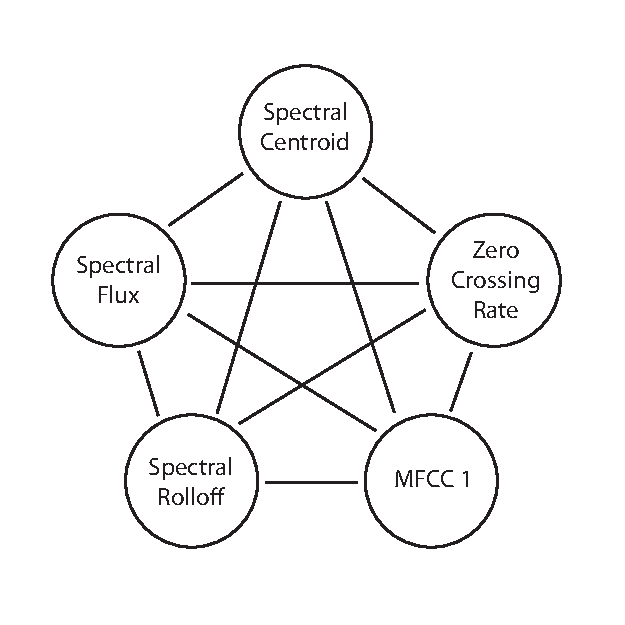
\includegraphics[width=0.3\textwidth]{figures/featGraph.pdf}
\end{center}

Consider a graph whose nodes represent specific features that can be extracted from a song, e.g. spectral centroid, rolloff, etc.  The goal is to connect the nodes with weighted edges such that features can vote for other features if they believe it is important.  More specifically, we look for a similarity measure between features.  If two features are similar, then they will vote for each other.  Features with a lot of votes will then be selected with the page rank algorithm.  Since each song acts as an observation of the feature set, perhaps the most obvious choice for a similarity measure is correlation.  If two features are highly correlated (or anti-correlated), then we can say that they are similar.  Let $e_{ij}$ represent the edge from node $i$, corresponding to feature $f_i$, to node $j$, corresponding to feature $f_j$, and $w_{ij}$ be the corresponding weight of the edge, then
$$w_{ij} = \text{corr}(f_i,f_j)^2$$
We take the square correlation since we want both correlated and anti-correlated features to be considered similar.  The correlation we used is a Spearman correlation.  The benefit of Spearman over Pearson is that the Pearson correlation assumes a linear relationship, whereas Spearman is nonparametric and better accounts for nonlinearities.\\

Once we have constructed a matrix, $W$, containing all of the weights of our feature graph, we normalize the rows to sum to $1$, giving a normalized matrix $H$.  Our graph is naturally (nearly) fully connected with our choice of weights, so no escape probabilities need to be added to our matrix.  This also means that we do not need to include any damping that is often used with Page Rank.  Finding the rankings of the features is then just a simple eigenvalue problem, solving $r^T = r^T H$.  Running this ranking method on the full set of training songs gave us top 5 features shown in Table \ref{tab:all_pr}.\\

\begin{table}[!h]
\begin{center}
\begin{tabular}{|l|l|}
\hline
Rank & Feature \\ \hline
1 & Mfcc 1\tss{(1)} \\ \hline
2 & Spectral Flatness\tss{(1)} \\ \hline
3 & Peak Envelope Max\tss{(1)} \\ \hline
4 & Spectral Slope\tss{(1)} \\ \hline
5 & Autocorrelation Max\tss{(1)} \\ \hline
\end{tabular}
\caption{Top 5 features extracted using Page Rank with the entire feature set.  Superscripts refer to which moment of the feature is being considered (1-mean, 2-variance, 3-skewness, 4-kurtosis).}
\label{tab:all_pr}
\end{center}
\end{table}

One potential problem with this implementation is that all songs are considered to be representable by the same features.  In general, this is not true as different genres exhibit different behaviors of features.  To capture this difference between features, we can instead run the feature selection considering a single genre at a time.  The top 5 features for each genre are shown in Table \ref{tab:genre_pr}.\\

\begin{table}[!h]
\begin{center}
\begin{tabular}{|l|l|l|l|}
\hline
Rank & Classical & Electronic & Jazz/Blues \\ \hline
1 & Zero Crossing Rate\tss{(1)} & Spectral Slope\tss{(1)} & Spectral Rolloff\tss{(2)} \\ \hline
2 & Spectral Centroid\tss{(1)} & MFCC 1\tss{(1)} & MFCC 3\tss{(2)} \\ \hline
3 & Spectral Spread\tss{(1)} & RMS\tss{(1)} & FP DLF \\ \hline
4 & Spectral Rolloff\tss{(1)} & Peak Envelope\tss{(1)} & MFCC 5\tss{(1)} \\ \hline
5 & Spectral Crest\tss{(1)} & Spectral Flux\tss{(1)} & FP Bass \\ \hline
\hline
Rank & Metal/Punk & Rock/Pop & World \\ \hline
1 & MFCC 4\tss{(2)} & Spectral Flatness\tss{(1)} & MFCC 1\tss{(1)} \\ \hline
2 & Spectral Crest\tss{(1)} & MFCC 1\tss{(1)} & Predicitivity Ratio\tss{(1)} \\ \hline
3 & Predictivity Ratio\tss{(1)} & Predictivity Ratio\tss{(1)} & Spectral Flatness\tss{(1)}\\ \hline
4 & Peak Envelope\tss{(4)} & Spectral Crest\tss{(1)} & Spectral Crest\tss{(1)} \\ \hline
5 & MFCC 1\tss{(4)} & Spectral Spread\tss{(1)} & Spectral Spread\tss{(1)} \\ \hline
\end{tabular}

\caption{Top 5 features extracted using Page Rank with the genres considered separately.  Superscripts refer to which moment of the feature is being considered (1-mean, 2-variance, 3-skewness, 4-kurtosis).}
\label{tab:genre_pr}
\end{center}
\end{table}

%\begin{figure}[!ht]
%\begin{center}
%\vspace{-1in}
%\includegraphics[width=0.6\textwidth]{figures/genrePR.pdf}
%\vspace{-1in}
%\caption{Relationship between dimension and classification accuracy using features selected with Page Rank and a kNN classifier.}
%\end{center}
%\end{figure}

The downside to using correlation as a similarity measure is that highly correlated features will often be selected around similar times.  This is less than ideal as we would want to select features that have a lot of information, and exclude features that contain the same information.  In order to attempt to solve this issue, we tried a step-by-step feature selection method, where after a feature is selected, the corresponding node is removed from the graph, and a penalty added to features that have high correlation to the selected feature.

\hrulefill

\textbf{Algorithm:} Feature at a time Page Rank
\begin{itemize}
\item Construct a matrix, $W$, of edge weights, where $W_{ij} = \text{corr}(f_i,f_j)^2$
\item Create a matrix, $H$, with rows being the normalized (sum to 1) rows of $W$
\item Repeat:
\begin{itemize}
\item Calculate the left eigenvector, $r^T = r^T H$
\item Find the feature with the highest ranking, $\ell = \argmax_i\{r_i\}$
\item Rescale $W$ by $W_{ij} = W_{ij} (1 - \alpha W_{j\ell})$
\item Remove row and column $\ell$ from $W$
\item Recalculate $H$
\end{itemize}
\end{itemize}
\hrulefill

Unfortunately, this adjustment generally performs worse.  Initially it gives slightly better performance, but then quickly drops below the all at once Page Rank method.

\begin{figure}[!h]
\begin{center}
\vspace{-1in}
\includegraphics[width=0.6\textwidth]{figures/adjPR.pdf}
\vspace{-1in}
\caption{Accuracy vs Dimension with both the all at once Page Rank and the feature at a time Page Rank (with optimal $\alpha$)}
\end{center}
\end{figure}

\subsection{Graph Methods and Spectral Clustering}
From the features that we extracted we have a feature vector for every training and test song that can be label as a set of data points $x_1,\hdots, x_n$. From the data points we create some notion of similarity $s_{ij} \geq 0$  between the data points $x_i$ and $x_j$. Using the Gaussian similarity function, 
\[s(x_i,x_j) = e^{\frac{-||x_i-x_j||^2}{2_\sigma^2}}\]
where the parameter $\sigma$ is chosen by the user, we can create a similarity matrix of all data points. We can then create a graph representation of the data using the similarity matrix. There are three ways that we use to create the similarity graphs. A graph $G(V,E)$ is undirected with the vertex set $V = \{ v_i, \hdots, v_n\}$ and the edge set $E$  with the property that if vertex $v_i$ is connected to $v_j$ the weighted edge $e_{i,j} = e_{j,j} \in E$.  

\begin{itemize}
\item {\bf{$\epsilon$-Neighborhood Graph:}} Choose a parameter $\epsilon$ and keep only the values of $s_{i,j}$ that are greater than $\epsilon$.  
\item {\bf{k-Nearest Neighbor Graph:}} We connect the vertex $v_i$ with the vertex $v_j$ if $v_j$ is among the $k$-nearest neighbors of $v_i$ with the edge weight $s_{ij}$. 
\item{\bf{Fully Connected Graph:}} We keep all the weighted edges with positive similarity $s_{ij}$. 
\end{itemize}

We can then define the adjacency matrix $W$ is as the matrix with the weighted edges that was chosen by the above methods. We can then define the graph Laplacian and the normalized graph Laplacian as 

\[ L = D -W\] and \[ \tilde{L} = I -D^{-1/2}WD^{-1/2}\] 
Where $D$ is the row sum of the weighted matrix. From the graph Laplacians we have a few methods of spectral clustering to choose from. 

\begin{itemize}
\item {\bf{ Unnormalized Spectral Clustering:}}
\begin{enumerate}
\item Computed the unnormalized graph Laplacian, $L$,from the similarity adjacency matrix.  
\item Compute the associated eigenvectors of the first (magnitude) $k$ eigenvalues of $L$ and store them in the matrix $V$. 
\item Using the rows of $V$  as our spectral coordinates for clustering the points. 
\end{enumerate}
 \item {\bf{ Normalized Spectral Clustering Method 1:}}
 \begin{enumerate}
\item Computed the unnormalized graph Laplacian $L$ from the similarity adjacency matrix.  
\item Compute the associated eigenvectors of the first (magnitude) $k$ eigenvalues of the system, $Lv = \lambda Dv$ and store them in the matrix $V$. 
\item Using the rows of $V$  as our spectral coordinates for clustering the points. 
\end{enumerate}

\item {\bf{ Normalized Spectral Clustering Method 2:}}
\begin{enumerate}
\item Computed the normalized graph Laplacian $L$ from the similarity adjacency matrix.  
\item Compute the associated eigenvectors of the first (magnitude) $k$ eigenvalues of $L$ and store them in the matrix $V$. 
\item Using the rows of $V$ normalize the row sums to have 1 and then use the normalized $V$ as our spectral  coordinates for clustering the points. 
\end{enumerate}

\end{itemize}



%_________________________________________________________________
\section{Statistical learning}
%Explain how the training data help find the genre of an unknown
%song. This could be as simple as finding the closest song among all
%the songs for which you know the genre. Or it could involve more
%sophisticated methods.
%_________________________________________________________________
\subsection{$k$-Nearest Neighbor}
Perhaps the simplest way to classify a new song is to use its $k$-nearest neighbors.  We first compute the reduced dimension feature vector of all the songs in the training set and the test song.  Then we find the $k$ songs in the training set that are closest in some metric to the test song.  We used the standardized Euclidean distance, but there are many other possible distances.  Finally, the method finds the most common genre (with ties broken in some manner) among the $k$-nearest neighbors and assigns that genre to the test song.\\

\subsection{Support Vector Machines}
Support vector machines (SVMs) are another supervised learning algorithm.  There were originally developed as a binary classification method, but there exist many methods to extend SVMs to support multiple classes.  In the linear case, the SVM method attempts to draw the ``best'' hyperplane between two sets of points with known classification.  The ``best'' hyperplane is the one that maximizes the margin between the two classes.  Sometimes the data are nearly linearly separable, but perhaps some of the points from one class live on the other side of what would otherwise be the maximum-margin separating hyperplane.  This issue is resolved by admitting these points and adding a penalty to account for the margin violation.\\

In more extreme cases, the data are truly non-linearly separable.  It may be possible to map the data to a higher dimensional space in which they are linearly separable.  However, determining suitable mappings can be quite difficult and may add considerable computational expense.  It turns out that we can implicitly map the data to a higher (even infinite) dimensional space using what is known as the kernel trick.  It transpires that a slight modification to the linear SVM algorithm gives us the advantage of working with the data mapped into a higher dimensional space all without actually computing the mapping!  The linear SVM algorithm uses the inner product $\mathbf{x}_i\cdot\mathbf{x}_j$ between data vectors $\mathbf{x}_i$ and $\mathbf{x}_j$; the kernel trick essentially just replaces the standard inner product with a new kernel.  Popular kernels are the Gaussian kernel

\[ k(\mathbf{x}_i,\mathbf{x}_j) = \exp\left(-\gamma \|\mathbf{x}_i-\mathbf{x}_j\|\right), \] 

\noindent where $\gamma>0$ is a chosen scale parameter, and the polynomial kernel

\[ k(\mathbf{x}_i,\mathbf{x}_j) = \left(1+\mathbf{x}_i\cdot\mathbf{x}_j\right)^p, \] 

\noindent where $p$ is a chosen polynomial order.\\

\subsubsection{Extension of SVMs to multiple classes}
In order to fully utilize SVMs as a classification method, they should be extended beyond a binary classifier.  There exist methods that ``natively'' extend the SVM ideas to support multiple classes.  Another approach, the one we take, is to build many binary SVM classifiers that, when combined in an intelligent manner, result in a multi-class classier.\\ 

Perhaps the simplest multi-class extension of binary SVMs is to use a ``one vs. all'' classification for each class.  This method builds an SVM classifier for each class and trains the classifier by grouping the training data into in the class and not in the class.  Specifically, if there are $n$ classes, we build the $n$ SVM classifiers $f_i$, $i=1,...,n$ that classify the data into class $i$ and not class $i$.  Each $f_i$ will return $1$ if the test data is likely in class $i$ and $0$ otherwise.  Table \ref{tab:onevall} shows a schematic of the return values for each $f_i$ for $n=6$.  To characterize a test song, we run each classifier, which will also produce a score measuring the likelihood that the song is in the class; we assign the most likely genre to the test song.\\

\begin{table}[h!]
   \centering
   \begin{tabular}{|c|cccccc|}
      \hline
      class&$f_1$ & $f_2$ & $f_3$ & $f_4$ & $f_5$ & $f_6$\\\hline
      1 & 1 & 0 & 0 & 0 &0 &0\\\hline
      2 & 0 & 1 & 0 & 0 & 0 & 0\\\hline
      3 & 0 & 0 & 1 & 0 & 0 & 0\\\hline
      4 & 0 & 0 & 0 & 1 & 0 & 0\\\hline
      5 & 0 & 0 & 0 & 0 & 1 & 0\\\hline
      6 & 0 & 0 & 0 & 0 & 0 & 1\\\hline
   \end{tabular}
   \caption{Schematic of SVM multi-class extension one-versus-all.}
   \label{tab:onevall}
\end{table}

Another popular option is the ``one vs. one'' extension, wherein one builds a classifier for each pair of classes.  If there are $n$ classes, then we will have $\binom n 2$ SVM classifiers.  Abusing notation slightly, let $f_{ij}$ be the classifier that decides between class $i$ and class $j$.  We set $f_{ij}$ to return $1$ if the test song likely belongs to class $i$ and $0$ if it likely belongs to class $j$.  See Table \ref{tab:onevone} for a schematic.  We if apply $f_{ij}$ to a song that does not belong to either class $i$ or class $j$, then the song will get mislabeled.  By applying each $f_{ij}$ to a test song, we get possibly multiple votes for each genre; we assign the genre with the most votes.\\

\begin{table}
   \centering
   \begin{tabular}{|c|ccccccc|}
      \hline
      class&$f_{12}$ & $f_{13}$ & $f_{14}$ & $f_{15}$ & $f_{16}$ & $f_{23}$ & $\cdots$ \\\hline
      1 & 1 & 1 & 1 & 1 & 1 &   & $\cdots$ \\\hline
      2 & 0 &   &   &   &   & 1 & $\cdots$ \\\hline
      3 &   & 0 &   &   &   & 0 & $\cdots$ \\\hline
      4 &   &   & 0 &   &   &   & $\cdots$ \\\hline
      5 &   &   &   & 0 &   &   & $\cdots$ \\\hline
      6 &   &   &   &   & 0 &   & $\cdots$ \\\hline
   \end{tabular}
   \caption{Schematic of SVM multi-class extension one-versus-one.}
   \label{tab:onevone}
\end{table}

The final extension method we consider, called error correcting output codes (ECOC), uses ideas borrowed from error control coding.  When we apply some SVM classifier $f_i$ to a test track, it might make an error, in effect switching a $1$ to a $0$ or a $0$ to a $1$.  This happens for each classifier $f_i$.  One can think of the sequence of outputs of the $f_i$ as the output of a noisy communications channel.  As an example, see Table \ref{tab:ecoc}, which shows a choice of $f_i$, $i=1,...,6$ based on a Hamming code.  To classify a new track, we run each classifier $f_i$ on the test track, resulting in a row vector.  We then compare the output row vector with each row of the table (which corresponds to the unique codeword assigned to a class) and pick the closest class based on the Hamming distance.\\

\begin{table}
   \centering
   \begin{tabular}{|c|cccccc|}
      \hline
      class&$f_{1}$ & $f_{2}$ & $f_{3}$ & $f_{4}$ & $f_{5}$ & $f_{6}$ \\\hline
      1 & 0 & 0 & 0 & 0 & 0 & 0 \\\hline
      2 & 0 & 1 & 0 & 1 & 0 & 1 \\\hline
      3 & 1 & 0 & 0 & 1 & 1 & 0 \\\hline
      4 & 1 & 1 & 0 & 0 & 1 & 1 \\\hline
      5 & 1 & 1 & 1 & 0 & 0 & 0 \\\hline
      6 & 1 & 0 & 1 & 1 & 0 & 1 \\\hline
   \end{tabular}
   \caption{Schematic of SVM multi-class extension based on a Hamming code.}
   \label{tab:ecoc}
\end{table}


%_________________________________________________________________
\section{Experiments}
%Describe the experiments, and include the confusion matrix. Discuss
%the influence of the various parameters, and describe how the optimal
%parameters were chosen. Include the computation time for your method.
%_________________________________________________________________

Our implementation of the algorithms presented above are hosted at \url{https://github.com/jamesfolberth/hdd_project}.\\

In this section we will describe a few of the experiments we performed.  We first computed and saved the feature vectors for the training set.  For our implementation, this is the performance bottleneck, and it took about three hours to compute the feature vectors for the training set.  This is due not to the complexity of extracting the features but due to our use of an inefficient toolbox (which we use for convenience); we believe that it is possible to optimize the routines in the toolbox we use for our purposes.\\

Once the feature vectors are computed, we can reduce dimension and attempt training and classification.  We first used PCA and LLE dimension reduction as a baseline for comparison against the PageRank feature selection.  For the sake of brevity, we only note that we were able to optimize the parameters of the PageRank feature selection to perform significantly better than both optimized PCA and optimized LLE.  We use both the $k$-nearest neighbor and multi-class SVM classifiers.  The $k$-nearest neighbor classifier generally works well with $k=5$ neighbors.  Generally, one-versus-all SVM and ECOC SVM with a Hamming-like code perform quite well with a polynomial kernel with order $p\approx 2.5$.  The one-versus-one SVM classifier did not perform as well as the other two multi-class extensions, and we found the Gaussian kernel did not work well.\\

One of the main parameters of the PageRank feature selection is how many features we select.  In Figure \ref{fig:prDim} we have plotted the classification accuracy during training cross-validation as a function of dimension using the one-versus-all SVM classifier with a genre-based PageRank feature selection.  Looking only at the aggregate adjusted classification rate, we see that the optimal dimensionality is around $125$ dimensions.  Looking at each genre we see that different genres obtain peak performance at different dimensionalities.

\begin{figure}[h!]
   \centering
   \includegraphics[width=0.45\textwidth]{figures/optimSVMOVAprDim_genre05_Dale.pdf}
   \includegraphics[width=0.45\textwidth]{figures/optimSVMOVAprDimClass_Dale.pdf}
   \caption{Dimension dependence of genre-based PageRank feature selection with one-versus-all SVM.}
   \label{fig:prDim}
\end{figure}

For the $125$ dimensional PageRank dimension reduced feature vectors, running a cross validation of the one-versus-all SVM classifier on the training set takes approximately $25$ seconds running in serial on a $1.6\,\text{GHz}$ CPU.  In Table \ref{tab:xval} we show the results of a cross-validation using the $125$ selected features and the one-vs-all SVM classifier.  The entries are normalized so that the column sums are $1$ (entry $(i,j)$ is the average rate that genre $j$ is classified as genre $i$).  The most significant confusions are between world and classical, rock/pop and metal/punk, and jazz/blues and rock/pop.  This cross-validation gave an adjusted classification rate of $73.1\%$, which matches what we expect from Figure \ref{fig:prDim}.\\

\begin{table}[h!]
   \centering
   \begin{tabular}{ l||l | l | l | l | l | l | }
   & classical& electronic& jazz\_blues& metal\_punk& rock\_pop& world\\\hline
   classical & $0.94 \pm0.03$ &$0.03 \pm0.04$ &$0.00 \pm0.00$ &$0.00 \pm0.00$ &$0.03 \pm0.04$ &$0.20 \pm0.07$ \\ \hline 
   electronic & $0.00 \pm0.01$ &$0.73 \pm0.09$ &$0.02 \pm0.07$ &$0.03 \pm0.05$ &$0.09 \pm0.07$ &$0.06 \pm0.04$ \\ \hline 
   jazz\_blues & $0.00 \pm0.00$ &$0.01 \pm0.01$ &$0.80 \pm0.17$ &$0.00 \pm0.00$ &$0.01 \pm0.02$ &$0.01 \pm0.02$ \\ \hline 
   metal\_punk & $0.01 \pm0.01$ &$0.01 \pm0.03$ &$0.00 \pm0.00$ &$0.60 \pm0.17$ &$0.09 \pm0.07$ &$0.04 \pm0.04$ \\ \hline 
   rock\_pop & $0.01 \pm0.01$ &$0.10 \pm0.06$ &$0.12 \pm0.12$ &$0.30 \pm0.16$ &$0.68 \pm0.10$ &$0.04 \pm0.04$ \\ \hline 
   world & $0.05 \pm0.02$ &$0.11 \pm0.06$ &$0.07 \pm0.10$ &$0.07 \pm0.08$ &$0.09 \pm0.07$ &$0.64 \pm0.08$ \\ \hline 
   \end{tabular}
   \caption{Confusion matrix (rescaled) for cross-validation using genre-based PageRank and one-vs-all SVM.}
   \label{tab:xval}
\end{table}

For the final test with PageRank, we attempt classification of the test data.  We use the optimal parameters found by running cross-validations.  Specifically, we use a genre-based PageRank feature selection keeping $125$ features and one-versus-all SVM with a polynomial kernel with order $p=2.5$.  Table \ref{tab:class} shows the confusion matrix for the classification, which has an adjusted classification rate of $97.3\%$.  The classification performs much better on the test data compared to during cross-validation.

\begin{table}[h!]
   \centering
   \begin{tabular}{ l||l | l | l | l | l | l | }
   & classical & electronic & jazz\_blues & metal\_punk & rock\_pop & world\\\hline
   classical & 25 &0 &0 &0 &0 &0 \\ \hline 
   electronic & 0 &25 &1 &0 &0 &0 \\ \hline 
   jazz\_blues & 0 &0 &24 &0 &0 &0 \\ \hline 
   metal\_punk & 0 &0 &0 &25 &0 &0 \\ \hline 
   rock\_pop & 0 &0 &0 &0 &24 &2 \\ \hline 
   world & 0 &0 &0 &0 &1 &23 \\ \hline 
   \end{tabular}
   \caption{Confusion matrix for test classification using genre-based PageRank and one-vs-all SVM.}
   \label{tab:class}
\end{table}


\subsection{Experiments for Graphs Methods} 
Using the optimal features that were selected using the PageRank algorithm we normalized each feature and created the similarity matrix using the Gaussian similarity function. After a number of tests we selected $\sigma = 0.15$. In the following graphs {\color{blue} blue} is the Unnormalized, {\color{red} red} is the Normalized Method 1 and {\color{green} green} represents the Normalized Method 2, using $k$-nearest neighbor classification with $k =5$. 
\begin{itemize}
\item{\bf{$\epsilon$-Neighborhood Graph:}} Using $\epsilon = 0.0338$ which is the mean of the similarity matrix we have the following results in Figure \ref{fig:G1}. We see that Normalized Method 2 outperformed the other two methods. 
\begin{figure}[h!]
   \centering
   \includegraphics[width=0.45\textwidth]{figures/G1_epsmean.png}
   \caption{$\epsilon$-Neighbor Graph}
   \label{fig:G1}
\end{figure}
\vspace{55mm}
\item{\bf{$k$-Nearest Neighborhood Graph:}} Below in Figure \ref{fig:G2} we have the results for each of the 3 methods of spectral clustering with the creation of the similarity graph using $k$-nearest neighbors with $k =2,3,5$. 
\begin{figure}[h!]
    \centering
        \begin{subfigure}[b]{0.45\textwidth}
                \includegraphics[width=\textwidth]{figures/G2_k_2.png}
   \caption{$k=2$}
    \end{subfigure}
    \begin{subfigure}[b]{0.45\textwidth}
                \includegraphics[width=\textwidth]{figures/G2_k_3_all.png}
      \caption{$k=3$}
          \end{subfigure}

      \begin{subfigure}[b]{0.45\textwidth}
                \includegraphics[width=\textwidth]{figures/G2_k_5_All.png}
      \caption{$k=5$}
          \end{subfigure}
   \caption{$k$-Nearest Neighbor Similarity Graph}
   \label{fig:G2}
\end{figure}
We can see that when $k=2$ with the Normalized Method 2 has the highest normalized probability correct. 
\vspace{55mm}
\item{\bf{Fully Connected Graph:}} Below in Figure \ref{fig:G3} we have the fully connected graph using all three methods. We see that the Unnormalized Method performed the best until we get to the higher number of eigenvectors and Normalized Method 2 performed the best. 
\begin{figure}[h!]
   \centering
   \includegraphics[width=0.45\textwidth]{figures/G3_All.png}
   \caption{Fully Connected Graph}
   \label{fig:G3}
\end{figure}
\end{itemize} 

Overall, the best results were for the $2$-Nearest Neighbor Graph with the Normalized Method 2 spectral clustering. Obviously, the PageRank feature selection and using one-versus-all SVM outperformed the graph methods. 
%_________________________________________________________________
\section{Discussion}
%Provide a critique of the approach and discuss any potential
%improvement. Discuss the ability of your approach to classify
%non-classical into the five remaining genres.
%_________________________________________________________________

One of the most critical steps in our approach is the selection of the original feature set.  We believe that we have populated our feature set with many powerful features.  For example, we have noticed that the inclusion of the WCH features generally improves the adjusted classification rate by a few percent.  Part of our approach is to create a feature set that is ``too large'' and then let an intelligent dimension reduction method trim down the dimensionality and remove less useful features.\\

As mentioned earlier, one potential problem with this approach is that the PageRank feature selection can provide less-than-optimal results via the selection of many highly correlated features.  We do not currently have a very good method of removing highly correlated features that do not add much new, useful information to our reduced feature set.  As an example of this effect, we included the WCH features from all sub-bands in our non-reduced feature set instead of just the $6$th and $7$th approximation and detail sub-bands.  The WCH features tend to be highly correlated across the sub-bands, as is hinted at in Figure \ref{fig:wch_box}.  When we include all WCH features and run a cross-validation with the optimal parameters for one-versus-all SVM mentioned in the Experiments section, we notice a significant decrease in classification rate.  Again, we suspect that this is due to the inclusion of too many highly correlated WCH features.\\

Other concerns are the dimensionality of the reduced feature space and the relative sizes of the training set to the testing set regarding the performance of the classification method.  The concern here is overfitting.  In our experiments with the genre-based PageRank feature selection with the one-versus-all SVM classifier, we found that the optimal dimensionality was about $125$ dimensions.  The parameters were chosen to optimize the classification rate during cross-validation.  Perhaps one reason the one-versus-one SVM classifier did not work as well is that each classifier is trained on a relatively small training set during cross-validation.  Compared to classical and world, there are very few jazz/blues songs; for example, the one-versus-one SVM classifier classifies jazz/blues about $30\%$ worse than the one-versus-all SVM classifier!  Thus, it seems that number of features is too high (at least for the one-versus-one SVM classifier) compared to the number of training songs.  The large jump in classification accuracy going from cross-validation to test song classification might also be explained by the increase in the number of training songs relative to feature dimensionality.\\

We have thought of a few improvements to our methods.  First, and perhaps the easiest, is to optimize the extraction of features from songs; this is by far the slowest part of our implementation.  We used the toolbox from the textbook \cite{lerch:aca}; the toolbox is designed to be instructive, not efficient.  We could also explore different error correcting codes to use in the multi-class extension of SVM.  The best error correcting code we used is a Hamming-like code where the codewords are separated by a Hamming distance of at least $7$.  Perhaps also we could use the SVM prediction score (which is used in the one-versus-all extension) as well as the binary output of each SVM classifier $f_i$.  In this manner we might be able to join the beneficial properties of the one-versus-all and ECOC extensions to SVM.  We have also explored a few ways of selecting features via a genre-based PageRank feature selection.  The best method we invented gives a \emph{slight} preference to some genres over others in the feature selection stage.  With some more creativity, perhaps one could find a better method to select features.  Also, it should be possible to build a binary tree classification method using a special feature selection and SVM classifier for each node.  This may also allow us to use fewer features per classifier, which hopefully will allow us to avoid overfitting and build a better classifier.\\

Finally, we would like to thank Dr. Meyer for his useful advice throughout the semester, particularly in regard to the WCH features.

% References
\bibliographystyle{siam}
\bibliography{mir}

\end{document}
